\documentclass{article}

% ==========================================
%           PACKAGES & DEFINITIONS
% ==========================================
\usepackage[utf8]{inputenc}
\usepackage[T1]{fontenc}
\usepackage{fancyhdr}
\usepackage{xcolor}
\usepackage[top=2.5cm,bottom=2.5cm, left=2.5cm, right=2.5cm]{geometry}
\usepackage{titlesec}
\usepackage{enumitem}
\usepackage{hyperref}
\usepackage{graphicx}
\usepackage{wrapfig}
\usepackage{setspace}
\usepackage{tabularx}
\usepackage{booktabs}
\usepackage{makecell}
\usepackage{changepage}
\usepackage{float}
\usepackage{microtype}
\usepackage{tcolorbox}
\usepackage{listings}
\tcbuselibrary{listings,breakable}

% --- Colors ---
\definecolor{dominantColor}{HTML}{000000}

% --- Section Formatting ---
\titleformat{\section}
{\color{dominantColor}\fontsize{22}{2.2em}\selectfont\bfseries}
{\thesection.}{0.3em}{}

\titleformat{\subsection}
{\color{dominantColor}\fontsize{18}{2.2em}\selectfont\bfseries}
{\thesubsection.}{0.3em}{}

% --- Header / Footer ---
\newcommand{\makeHeaderFooter}{
\thispagestyle{fancy}
\fancyhead{}
\rhead{} %\includegraphics[width=3cm]{pics/placeholder_logo.png}} % Placeholder for ESI or University logo
\lhead{} %\includegraphics[width=4cm]{pics/placeholder_logo.png}} % Placeholder for Project logo
\renewcommand{\headrulewidth}{0pt}
\fancyfoot{}
\cfoot{\fontsize{12pt}{1.2em}{\textbf{\today}}}
}

\hypersetup{
colorlinks,
linkcolor=black,
urlcolor=black
}

\setlength{\parindent}{0pt}
\setlength{\parskip}{1.2em}
\onehalfspacing

% --------------------------
% Python code style box
% --------------------------
\newtcblisting{pythoncode}[1][]{
    listing engine=listings,
    colback=black!95!white,
    colframe=black,
    coltitle=white,
    listing only,
    breakable,
    enhanced,
    sharp corners,
    boxrule=0.5mm,
    top=2mm, bottom=2mm, left=2mm, right=2mm,
    fonttitle=\bfseries,
    title=#1,
    listing options={
        language=Python,
        basicstyle=\ttfamily\footnotesize\color{white},
        keywordstyle=\color{cyan},
        commentstyle=\color{green!70!black},
        stringstyle=\color{orange},
        showstringspaces=false,
        breaklines=true
    }
}

% ==========================================
%               DOCUMENT
% ==========================================
\begin{document}

% ==========================================
%               TITLE PAGE
% ==========================================
\begin{titlepage}
\vspace*{\fill}

{\color{dominantColor}\hrule}
\vspace{0.6cm}

\begin{center}
\fontsize{40pt}{1.2em}\selectfont\textbf{Project Report}
\end{center}

\vspace{0.6cm}
{\color{dominantColor}\hrule}
\vspace{0.8cm}

\begin{center}
\fontsize{21pt}{1.4em}\selectfont
\textbf{Theme: Fine-Tuning Gemma 4 for Children's Story Generation}
\end{center}

\vspace{0.6in}

\begin{center}
\fontsize{19pt}{1.4em}\selectfont
This NLP project focuses on domain adaptation by fine-tuning Google's Gemma 4 (E2B-IT) model using QLoRA to generate educational and engaging children's stories. The pipeline includes model quantization, merging, and deployment using GGUF for efficient local inference.
\end{center}

\vspace{0.6in}

\begin{center}
\fontsize{17pt}{1.35em}\selectfont
\textbf{Group Members:} \\[0.3cm]
Benhammadi Lokmane \\[0.3cm]
Khedim Youcef \\[0.3cm]
% Add additional team members here
\end{center}

\vspace*{\fill}
\makeHeaderFooter
\end{titlepage}

% ==========================================
%               CONTENT
% ==========================================
\newpage
\pagestyle{fancy}
\fancyhf{}
\fancyhead[L]{NLP Project Report}
\fancyhead[R]{\thepage}

\tableofcontents
\newpage
\listoffigures
\newpage

% ==========================================
%               SECTIONS
% ==========================================

\section{Introduction and Problem Statement}
\label{sec:intro}

\subsection{The Challenge: Domain-Specific Text Generation}
Large Language Models (LLMs) are incredibly capable zero-shot generalists. However, when tasked with creating highly specific content—such as educational stories tailored to exact age groups—they often drift into generic language, hallucinate complex vocabulary, or fail to adhere to structural constraints.

Two primary challenges define this project:
\begin{itemize}[noitemsep, topsep=0pt]
    \item \textbf{Style Adaptation:} Adjusting the model's tone to be engaging, safe, and comprehensible for young children, categorized strictly by age levels.
    \item \textbf{Resource Constraints:} Fine-tuning billions of parameters requires substantial compute memory. Developing a pipeline capable of running on accessible hardware (like Kaggle's dual T4 GPUs) is critical.
\end{itemize}

\subsection{Our Approach: QLoRA Fine-Tuning and Edge Deployment}
We fine-tune Google's \texttt{gemma-4-E2B-it} model on a curated children's story dataset. To bypass hardware limitations, we utilize 4-bit Quantized Low-Rank Adaptation (QLoRA). Once trained, the adapters are merged back into the base model and converted into a highly optimized \texttt{.gguf} format, enabling fast, local inference on edge devices via \texttt{llama.cpp}.

\begin{figure}[H]
\centering
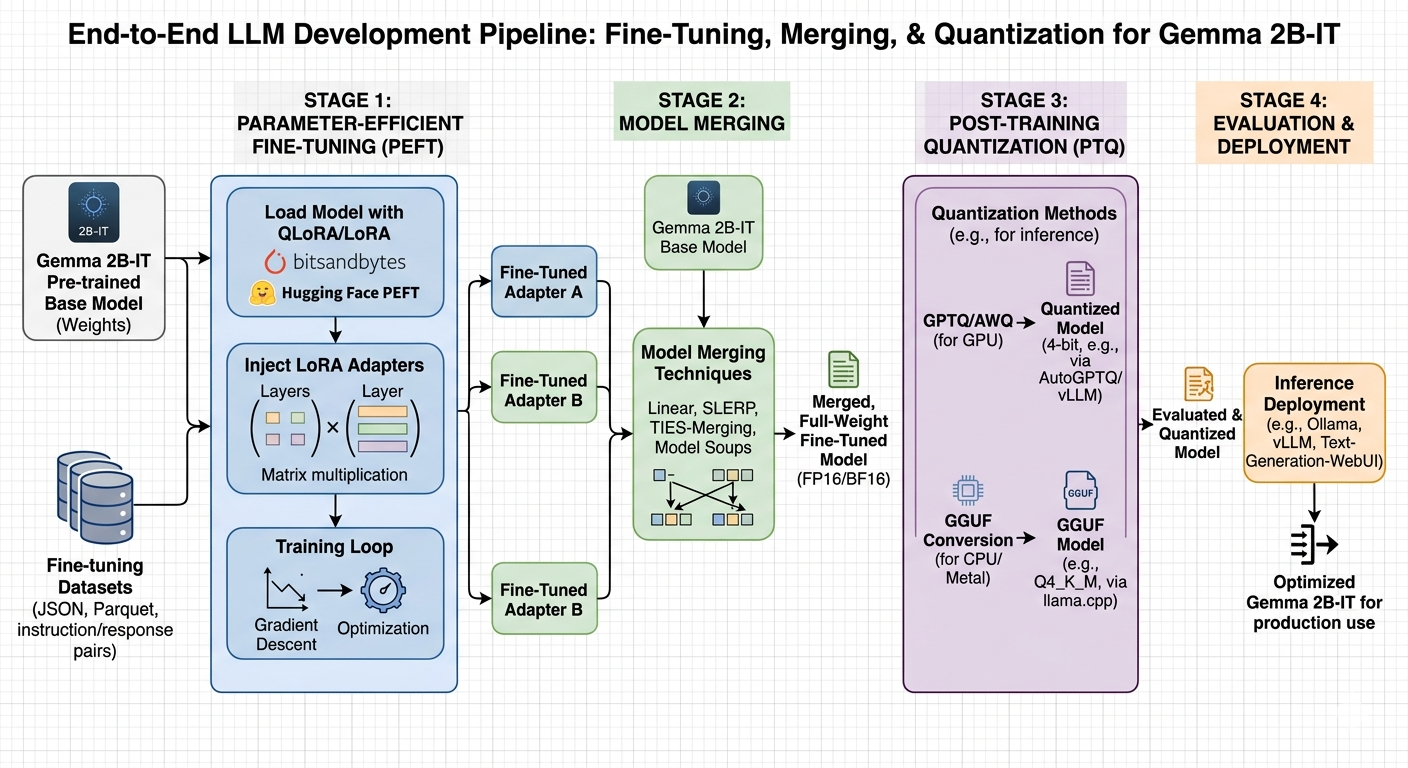
\includegraphics[width=1\textwidth]{pics/EndToEndLLMfinetuning.png} 
\caption{End-to-end LLM fine-tuning, merging, and quantization pipeline.}
\label{fig:pipeline}
\end{figure}

\clearpage
\newpage

\section{Background: Parameter-Efficient Fine-Tuning}
\label{sec:background}

\subsection{The Memory Bottleneck}
Training an LLM requires memory for model weights, gradients, optimizer states, and activations. A 2-billion parameter model in 16-bit precision requires roughly 4GB just to hold the weights, but over 16GB to train fully. This makes full fine-tuning inaccessible for consumer GPUs.

\subsection{Quantization and QLoRA}
To solve this, we employ **QLoRA**. The base model is loaded in 4-bit precision (NF4), drastically reducing the memory footprint. Instead of updating the original weights, QLoRA injects small, trainable "adapter" matrices into the model's layers. During training, only these adapter weights are updated while the base model remains frozen.

\begin{figure}[H]
\centering
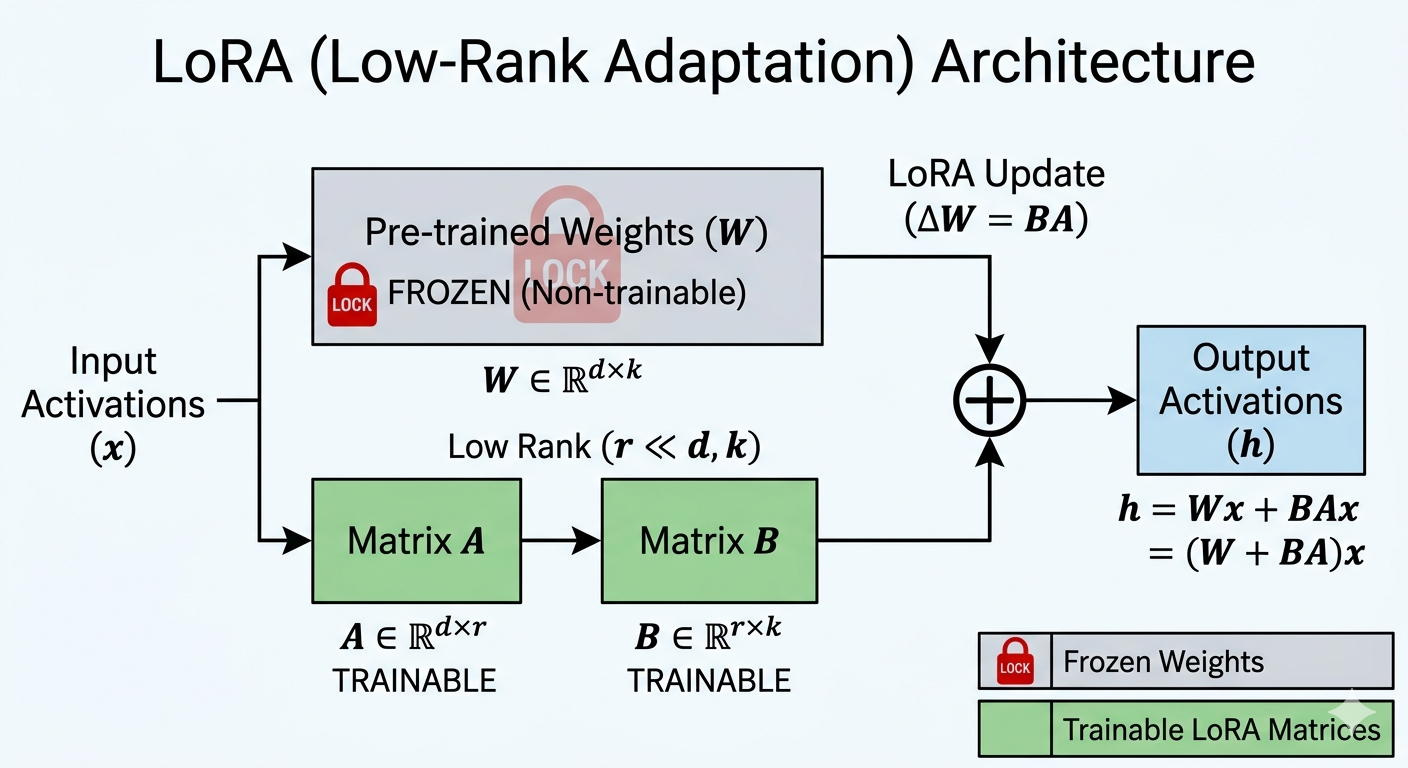
\includegraphics[width=0.8\textwidth]{pics/LoRAarch.png}
\caption{LoRA architecture: small rank decomposition matrices are trained while the pre-trained weights remain frozen.}
\label{fig:lora}
\end{figure}

\clearpage
\newpage

\section{Model Architecture: Gemma 4}
\label{sec:model}

\subsection{Overview of Gemma 4 E2B-IT}
Gemma is a family of lightweight, state-of-the-art open models built from the same research and technology used to create Google's Gemini models. We selected the \texttt{gemma-4-E2B-it} (Instruction Tuned) variant, which features an effective parameter count of 2.3 billion.

\subsection{Why Gemma 4 E2B?}
Three reasons drove this selection:
\begin{itemize}[noitemsep, topsep=0pt]
    \item \textbf{High Capacity-to-Size Ratio:} At 2.3B effective parameters, it offers deep reasoning capabilities while remaining small enough to fit comfortably on a single 16GB GPU during training.
    \item \textbf{Instruction Tuning:} The base model is already aligned to follow instructions and multi-turn conversations, meaning it requires less training data to learn the formatting of a prompt-response task.
    \item \textbf{Massive Vocabulary:} The model possesses a vocabulary size of 256,000 tokens, giving it exceptional multilingual and structural generation capacity.
\end{itemize}

\clearpage
\newpage

\section{Dataset}
\label{sec:dataset}

\subsection{Source and Formatting}
We utilized the \texttt{ajibawa-2023/Children-Stories-Collection} dataset from HuggingFace. The dataset consists of story prompts and corresponding stories suitable for children. 

To teach the model to adapt its vocabulary, we prefixed each prompt with an age-level constraint. The training samples were formatted into Gemma's native instruction format:

\begin{lstlisting}[language=json, breaklines=true, basicstyle=\small\ttfamily]
<start_of_turn>user
Level: Age5-6 - Short sentences.
Write a story about a brave little toaster.<end_of_turn>
<start_of_turn>model
Once upon a time, there was a little silver toaster. He lived in a warm kitchen...<end_of_turn>
\end{lstlisting}

\subsection{Dataset Statistics}
We subsampled 10,000 stories for this fine-tuning pass, splitting 95\% for training and 5\% for evaluation. 

\begin{figure}[H]
\centering
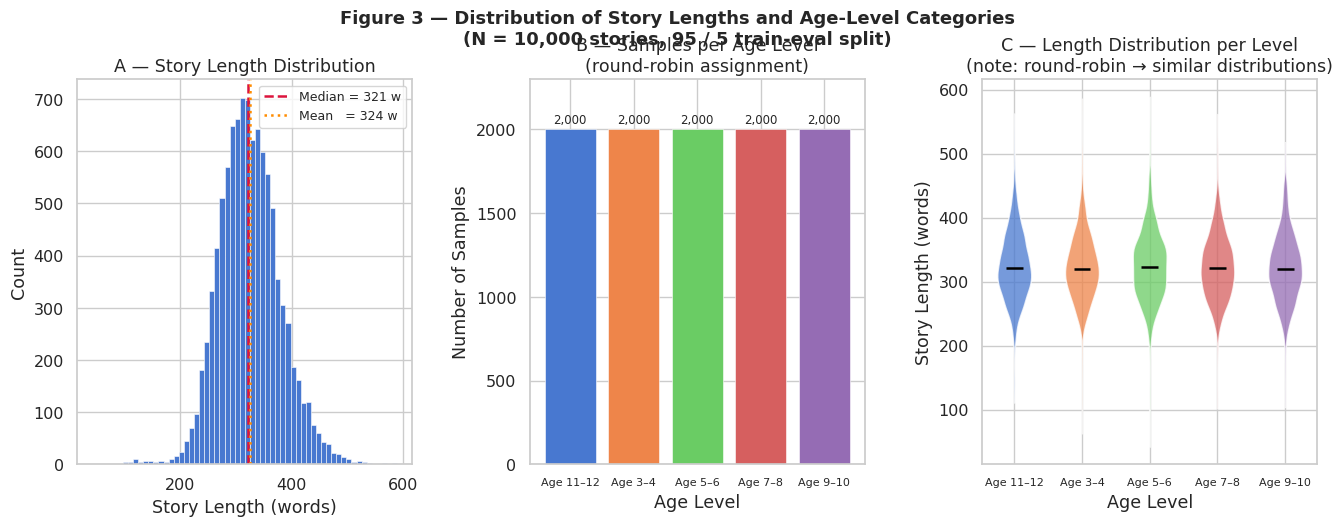
\includegraphics[width=0.8\textwidth]{pics/DatasetPlots.png} % PLACEHOLDER
\caption{Distribution of story lengths and age-level categories in the training sample.}
\label{fig:dataset_stats}
\end{figure}

\clearpage
\newpage

\section{Training Methodology}
\label{sec:training}

\subsection{Configuration and Hardware}
Training was orchestrated using the HuggingFace \texttt{Trainer} API on a Kaggle environment equipped with dual NVIDIA T4 GPUs. 

Key training parameters:
\begin{pythoncode}[Training Arguments]
training_args = TrainingArguments(
    per_device_train_batch_size=1,
    gradient_accumulation_steps=16,
    optim='paged_adamw_8bit',
    learning_rate=2e-4,
    fp16=True,
    gradient_checkpointing=True,
    eval_strategy='no' # Disabled to prevent OOM
)
\end{pythoncode}

\subsection{Overcoming Memory Constraints}
Due to Gemma 4's massive 256K token vocabulary, calculating cross-entropy loss over large sequences creates a massive memory spike. We mitigated this by:
\begin{enumerate}
    \item Enforcing \texttt{batch\_size = 1} with high gradient accumulation (16 steps) to simulate a batch size of 16.
    \item Enabling \texttt{gradient\_checkpointing} to trade computation time for VRAM savings.
    \item Setting \texttt{PYTORCH\_CUDA\_ALLOC\_CONF=expandable\_segments:True} to prevent CUDA memory fragmentation.
\end{enumerate}

\begin{figure}[H]
\centering
%\includegraphics[width=\textwidth]{pics/placeholder_training_curves.png} % PLACEHOLDER
\caption{Training loss curve over the 1-epoch fine-tuning run.}
\label{fig:loss_curve}
\end{figure}

\clearpage
\newpage

\section{Model Export and Deployment}
\label{sec:export}

\subsection{Merging the Adapters}
QLoRA results in standalone adapter weights. For efficient deployment, we reloaded the base model in FP16 precision on the CPU, injected the LoRA weights, and invoked \texttt{merge\_and\_unload()} to fuse them permanently.

\subsection{GGUF Quantization via llama.cpp}
To deploy the model locally, we converted the merged model into the GGUF (GPT-Generated Unified Format) standard using \texttt{llama.cpp}. 
The FP16 model was further quantized down to \texttt{Q4\_K\_M} (4-bit, medium quantization). This reduced the model's disk footprint to approximately 1.5 GB, allowing it to run entirely on consumer CPU RAM with minimal loss in generative quality.

\begin{figure}[H]
\centering
%\includegraphics[width=0.85\textwidth]{pics/placeholder_gguf.png} % PLACEHOLDER
\caption{The llama.cpp conversion and quantization process log.}
\label{fig:gguf}
\end{figure}

\clearpage
\newpage

\section{Evaluation and Results}
\label{sec:results}

\subsection{Qualitative Examples}
Post fine-tuning, the model reliably adhered to the age-level prefixes, adjusting its sentence complexity and vocabulary seamlessly. 

\begin{figure}[H]
\centering
%\includegraphics[width=0.9\textwidth]{pics/placeholder_generation.png} % PLACEHOLDER
\caption{Comparison of generated stories for Age 3-4 vs Age 11-12 from the same prompt.}
\label{fig:generations}
\end{figure}

\clearpage
\newpage

\section{Discussion and Limitations}

While the fine-tuned model successfully generated formatted, age-appropriate children's stories, several challenges and limitations remain:
\begin{itemize}[noitemsep, topsep=0pt]
    \item \textbf{Vocabulary Size Overhead:} The 256k vocabulary size of Gemma 4 makes cross-entropy loss computation extremely expensive in VRAM, restricting training batch sizes and evaluation strategies.
    \item \textbf{Catastrophic Forgetting:} By fine-tuning purely on children's stories, the model's general instructional capability may degrade outside of this specific domain.
    \item \textbf{Hallucinations:} Without grounding constraints, the model may occasionally generate nonsensical plot resolutions. Future work could involve RAG (Retrieval-Augmented Generation) to ground the stories in specific educational facts.
\end{itemize}

\clearpage
\newpage

\section{Technologies Used}

\subsection{PyTorch \& Transformers}
\begin{minipage}{0.7\textwidth}
PyTorch powers the underlying tensor math, while the HuggingFace Transformers library handles model loading, tokenization, and the training loop abstraction.
\end{minipage}\hspace{.2in}
\begin{minipage}{0.25\textwidth}\centering
%\includegraphics[width=0.7\textwidth]{pics/tech/placeholder_pytorch.png} % PLACEHOLDER
\end{minipage}

\vspace{.15in}

\subsection{PEFT \& BitsAndBytes}
\begin{minipage}{0.7\textwidth}
The PEFT library manages the LoRA adapter injection, while BitsAndBytes enables the NF4 precision loading essential for QLoRA on consumer hardware.
\end{minipage}\hspace{.2in}
\begin{minipage}{0.25\textwidth}\centering
%\includegraphics[width=0.7\textwidth]{pics/tech/placeholder_peft.png} % PLACEHOLDER
\end{minipage}

\vspace{.15in}

\subsection{llama.cpp}
\begin{minipage}{0.7\textwidth}
Written in pure C/C++, llama.cpp provides the engine for converting the PyTorch model into the highly optimized GGUF format for edge inference.
\end{minipage}\hspace{.2in}
\begin{minipage}{0.25\textwidth}\centering
%\includegraphics[width=0.5\textwidth]{pics/tech/placeholder_llama.png} % PLACEHOLDER
\end{minipage}

\vspace{.15in}

\subsection{Kaggle}
\begin{minipage}{0.7\textwidth}
Kaggle's cloud environment, specifically the dual T4 GPU accelerators, served as the primary hardware infrastructure for the fine-tuning process.
\end{minipage}\hspace{.2in}
\begin{minipage}{0.25\textwidth}\centering
%\includegraphics[width=0.7\textwidth]{pics/tech/placeholder_kaggle.png} % PLACEHOLDER
\end{minipage}

\end{document}
